\documentclass[conference]{IEEEtran}
\usepackage{cite}
\usepackage{amsmath,amssymb,amsfonts}
\usepackage{algorithmic}
\usepackage{graphicx}
\usepackage{textcomp}
\usepackage{xcolor}
\usepackage{subfig}
\usepackage{siunitx}
\usepackage{hyperref}
\usepackage{bm}
\usepackage{float}
\usepackage{url} % Added for \url command
\pagestyle{plain}
\usepackage{setspace}
\setlength{\textfloatsep}{10pt plus 1.0pt minus 2.0pt}
\setlength{\floatsep}{10pt plus 1.0pt minus 2.0pt}
\setlength{\intextsep}{10pt plus 1.0pt minus 2.0pt}

% Configure hyperref for colored links (using the blue from the slides)
\definecolor{myblue}{RGB}{0, 153, 204}
\hypersetup{
    colorlinks=true,
    linkcolor=myblue,
    filecolor=magenta,
    urlcolor=myblue,
    citecolor=green
}

\sisetup{per-mode=symbol} % For units like kHz

\begin{document}

\title{Modernizing the Theremin: A Portable Circuit with Single-Antenna and Manual Volume Knob}

% Adjust author names and details as needed
\author{\IEEEauthorblockN{Krish Pandya}
\IEEEauthorblockA{\textit{2023102026} \\
\textit{IIIT Hyderabad}\\
krish.pandya@students.iiit.ac.in} % Placeholder email
\and
\IEEEauthorblockN{Vaibhav Wadhwani}
\IEEEauthorblockA{\textit{2023102058} \\
\textit{IIIT Hyderabad}\\
vaibhav.wadhwani@students.iiit.ac.in} % Placeholder email
}

\maketitle

\begin{abstract}
    This report details the design, simulation, and testing of a modernized portable Theremin, an electronic musical instrument played without physical contact. Unlike traditional Theremins, our design features a single antenna for pitch control and a manual potentiometer for volume adjustment, making it more compact and accessible. The circuit utilizes capacitive sensing via the antenna to control the pitch of the output sound, with the core principle involving heterodyning signals from a Variable Frequency Oscillator (VFO) and a Fixed Frequency Oscillator (FFO). The resulting difference frequency, falling within the audible range, is then filtered, amplified, and output through a power amplifier stage. The design primarily uses operational amplifiers for oscillation, mixing, filtering, and pre-amplification, with a Class AB BJT stage for power amplification. Operating on a ±5V dual power supply derived from batteries, the circuit is completely portable and ready for use in various performance settings.
\end{abstract}

\section{Introduction}
The Theremin, invented by Léon Theremin around 1920, stands as one of the earliest electronic musical instruments and is unique for being played without physical contact. It typically features two antennas: one controlling pitch and the other controlling volume, based on the proximity of the player's hands \cite{theremin_wiki}. The instrument operates on the principle of heterodyning, where two high-frequency radio signals are mixed together. The difference between these two frequencies results in a beat frequency within the audible range (20 Hz to 20 kHz). Traditional Theremins typically feature two antennas: one controlling pitch and the other controlling volume, based on the proximity of the player's hands. Our modernized approach simplifies this design by using a single antenna for pitch control and incorporating a manual potentiometer for volume adjustment, making the instrument more portable and user-friendly.

The use of heterodyning is advantageous because LC oscillators, commonly used in such circuits, exhibit greater stability and precision at higher frequencies (hundreds of kHz to MHz range). Generating stable audio-frequency tones directly using simple LC circuits can be challenging and less accurate. By generating two higher frequencies—one fixed (FFO) and one variable (VFO) controlled by hand capacitance—and then mixing them, a precisely controllable audio frequency ($f_{VFO} - f_{FFO}$) can be obtained. The player's hand acts as the grounded plate of a variable capacitor relative to the pitch antenna, altering the capacitance in the VFO circuit and thus changing its frequency.

This project focuses on the design, simulation, and implementation of a portable Theremin circuit using readily available components like operational amplifiers (Op-Amps) and bipolar junction transistors (BJTs). While traditional Theremins use a second antenna for volume control, this design employs a potentiometer for manual volume adjustment.

\section{Working Principle}
The operation of the designed Theremin circuit relies on several key principles:
\begin{itemize}
    \item \textbf{Capacitive Sensing}: The player's hand acts as a variable capacitor when brought near the pitch antenna. This change in capacitance modifies the frequency of the Variable Frequency Oscillator (VFO).
    \item \textbf{Oscillation}: Two oscillators are used:
        \begin{itemize}
            \item \textbf{Variable Frequency Oscillator (VFO)}: Its frequency changes based on the hand's proximity to the pitch antenna.
            \item \textbf{Fixed Frequency Oscillator (FFO)}: Generates a stable reference frequency close to the VFO's operating range.
        \end{itemize}
    \item \textbf{Heterodyning (Mixing)}: The signals from the VFO and FFO are combined using a mixer circuit (summing amplifier). The output of the mixer contains sum ($f_{VFO} + f_{FFO}$) and difference ($|f_{VFO} - f_{FFO}|$) frequencies.
    \item \textbf{Filtering}: Active filters (low-pass and high-pass) are employed to isolate the difference frequency, which constitutes the audible tone, and remove unwanted DC offsets and high-frequency components.
    \item \textbf{Amplification and Volume Control}: The filtered audio signal is amplified. A potentiometer is integrated to allow manual control over the final output volume before the signal is sent to the power amplifier.
    \item \textbf{Power Amplification}: A Class AB power amplifier stage provides sufficient current gain to drive a low-impedance load, such as a speaker.
\end{itemize}

\section{Circuit Overview}
The complete Theremin circuit designed and simulated in LTSpice is shown in Fig.~\ref{fig:circuit_overview}. It integrates several functional blocks: the VFO, FFO, Mixer, Filters, Pre-Amplifier/Volume Control, Sound Amplifier, and Power Amplifier. Operational amplifiers (OP27, UA741, OP37) are utilized for most signal generation and processing stages. The circuit is powered by a $\pm$5V dual rail supply, typically derived from batteries using voltage regulators ( Note: We used give power supply, also tested using batteries , so it is completely portable and ready to use). Fig.~\ref{fig:physical_circuit_overview} shows a representation related to the physical implementation.

We have written almost all the formulas that we used in circuit, for further derivations and calculations, please refer to the slides ( Available on Github ) \cite{Github} . The circuit is designed to be compact and efficient, with careful consideration of component values to achieve the desired frequency response and gain characteristics. (Note: In the report the numbers you see with R and C, they can be cross-referenced with the circuit diagram, and these values can be seen in the circuit diagram \ref{fig:circuit_overview}, that can also be found on github as it's LTSpice file as well as images).

\begin{figure}[htbp]
    \centering
    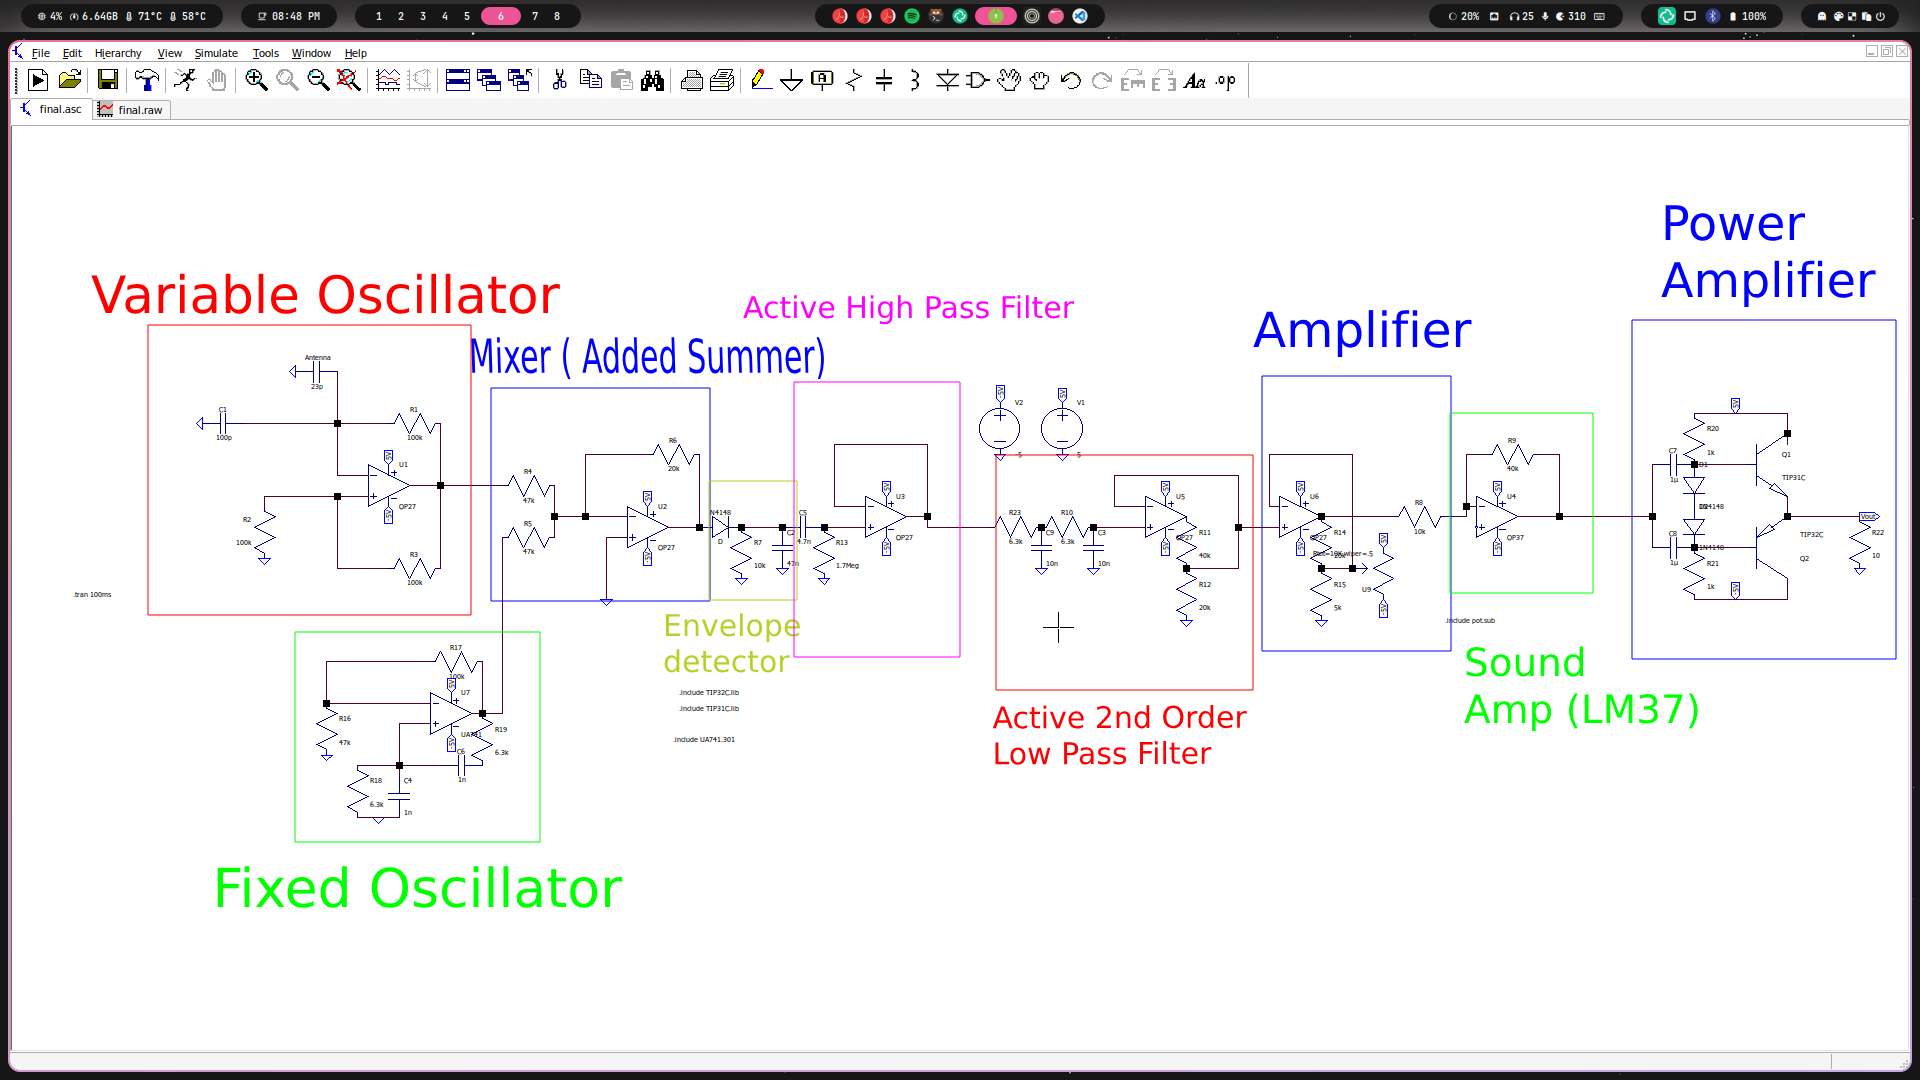
\includegraphics[width=0.95\linewidth]{theremin_circuit.png} % Ensure this image file is in the same directory or provide path
    \caption{Simulated Theremin Circuit Schematic (LTSpice)}
    \label{fig:circuit_overview}
\end{figure}

\begin{figure}[htbp]
    \centering
    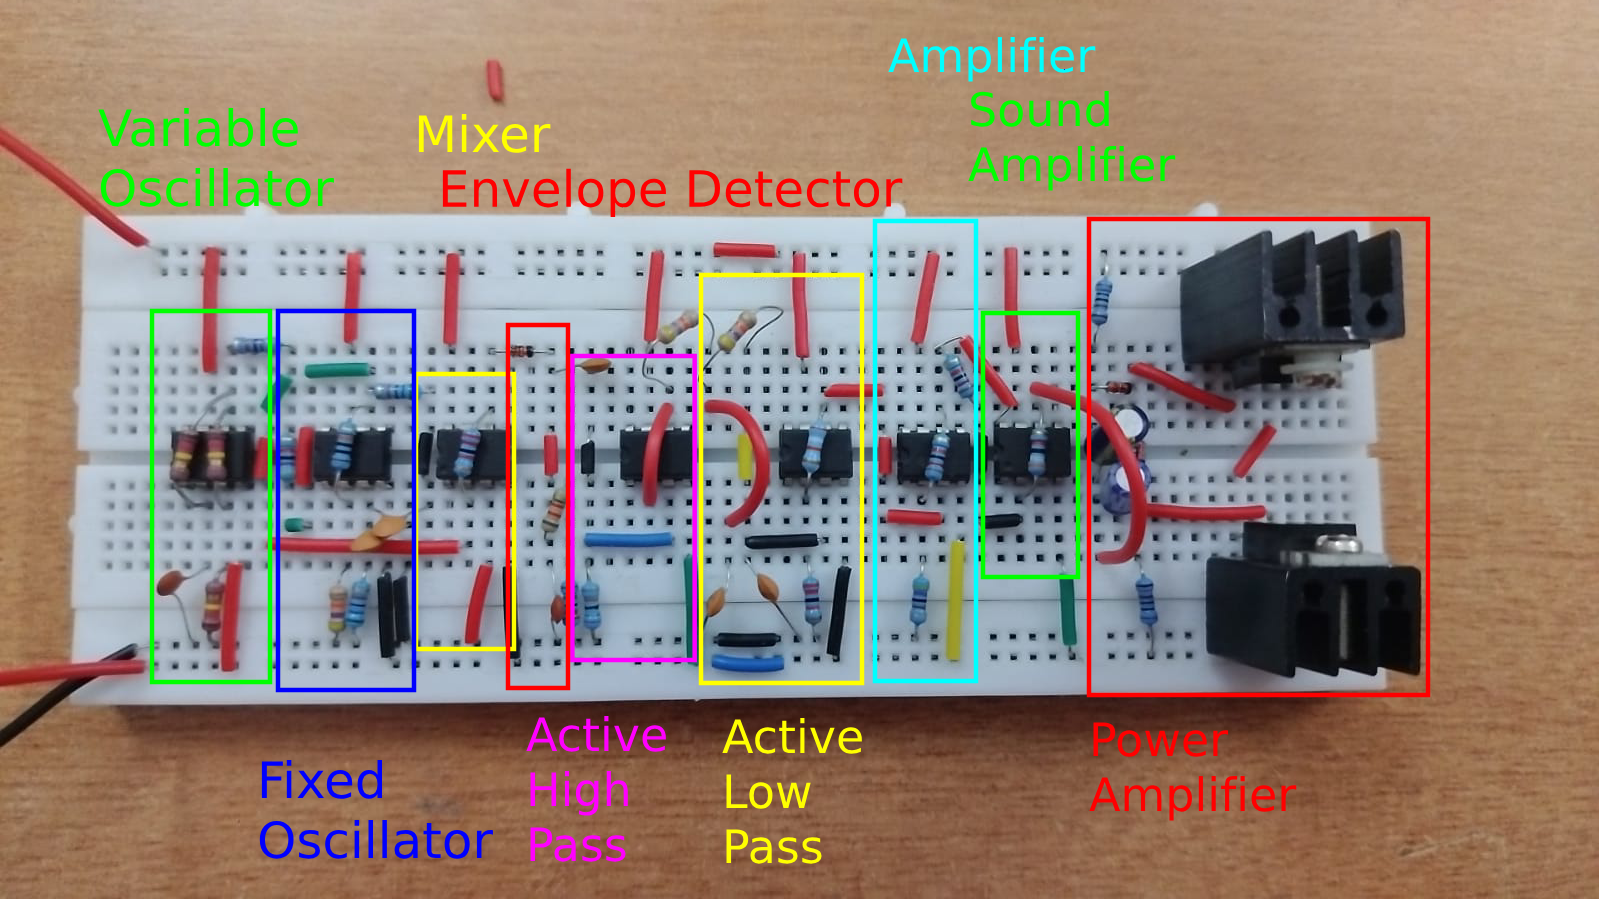
\includegraphics[width=0.95\linewidth]{physical_cirucit.png} % Ensure this image file is in the same directory or provide path
    \caption{Theremin Circuit Schematic (Physical Layout/Simplified)}
    \label{fig:physical_circuit_overview}
\end{figure}

\section{Oscillator Stages}

\subsection{Variable Frequency Oscillator (VFO)}
The VFO generates a signal whose frequency is sensitive to the capacitance of the pitch antenna, which varies with hand proximity.
\begin{itemize}
    \item \textbf{Topology}: An Op-Amp based relaxation oscillator using U1 (OP27) was chosen \cite{relax_osc}.
    \item \textbf{Key Components}: U1 (OP27), R1, R2, R3 (\SI{100}{\kilo\ohm}), C1 (\SI{100}{\pico\farad}), Antenna (modeled as \SI{23}{\pico\farad} base capacitance + variable hand capacitance $C_{hand}$) (Note: This can vary , ours was a copper wire around 600cm coiled up , so it came around this from frequency calculation.).
    \item \textbf{Operation}: The total capacitance ($C_{total} = C_{base} + C_{hand}$) at the oscillator's timing node determines its frequency. As the hand approaches the antenna, $C_{hand}$ increases, increasing $C_{total}$ and thus decreasing the VFO frequency $f_{VFO}$. Due to heterodyning, a decrease in $f_{VFO}$ leads to an increase in the difference frequency ($|f_{VFO} - f_{FFO}|$), resulting in a higher audible pitch.
    \item \textbf{Frequency Calculation}: The approximate frequency of the relaxation oscillator is given by:
        \begin{equation}
            f_{VFO} \approx \frac{1}{2 R C_{total} \ln\left(\frac{1+k}{1-k}\right)}
        \end{equation}
        where $R$ involves resistors like R3, $C_{total}$ is the total capacitance including the antenna and C1 (specific calculation depends on exact topology implementation, e.g., R=120k, C=175p from slides gives ~21.9kHz), and $k = \frac{R2}{R1+R2}$. With R1=R2=\SI{100}{\kilo\ohm}, $k=0.5$, and $\ln(\frac{1+0.5}{1-0.5}) = \ln(3) \approx 1.1$. The exact values used in the physical circuit (R = 120k, C = 175p - base capacitance) give a slightly different calculated base frequency around \SI{21.92}{\kilo\hertz}.
\end{itemize}
The output waveform of the implemented variable oscillator is shown in Fig.~\ref{fig:Variable_Oscillator}.

\begin{figure}[htbp]
    \centering
    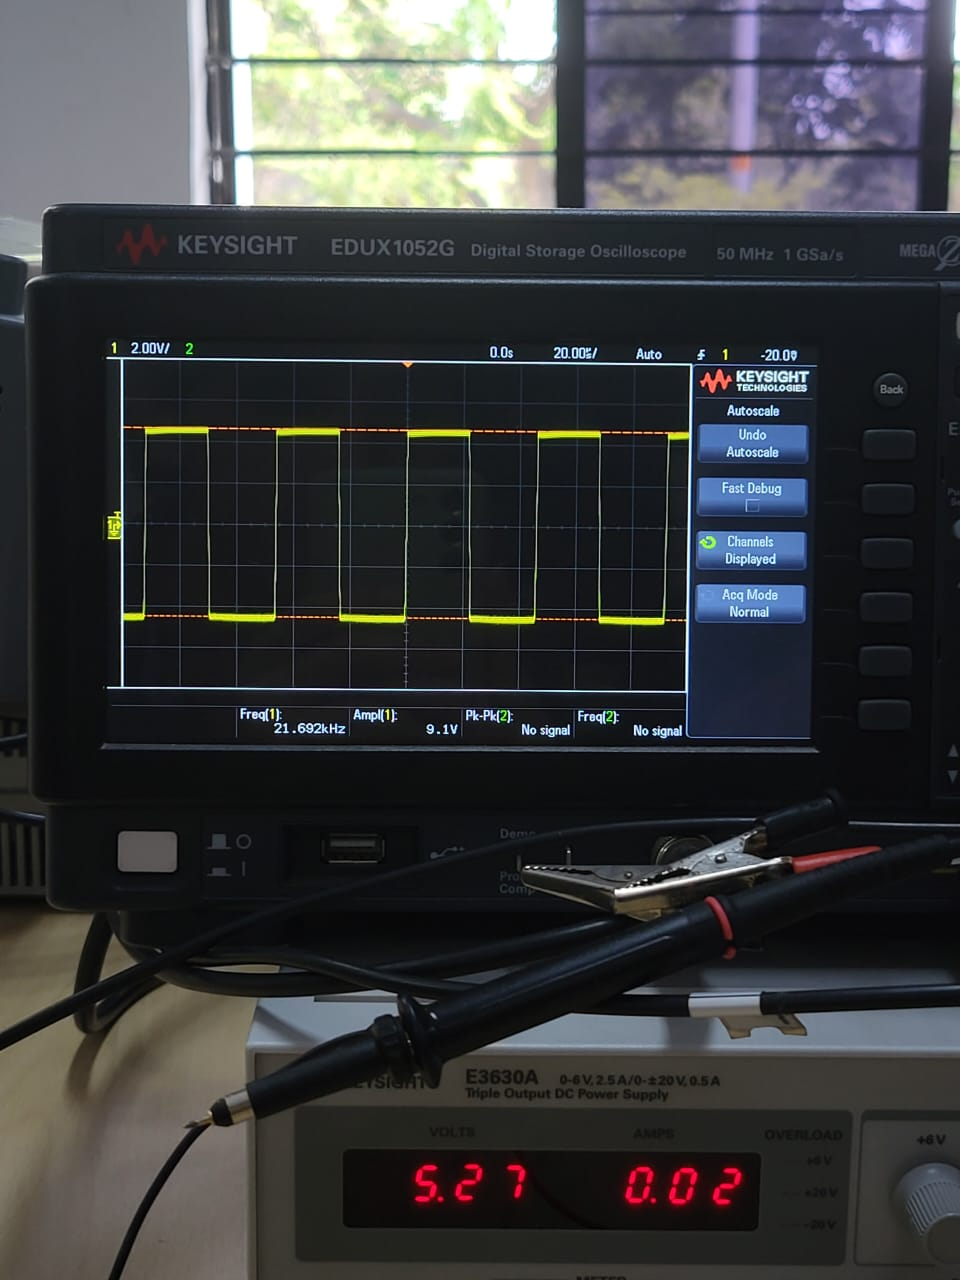
\includegraphics[width=0.8\linewidth]{variable.jpeg} % Ensure this image file is present
    \caption{Variable Oscillator Output Waveform (Physical Measurement)}
    \label{fig:Variable_Oscillator}
\end{figure}

\subsection{Fixed Frequency Oscillator (FFO)}
The FFO provides a stable reference frequency against which the VFO is compared.
\begin{itemize}
    \item \textbf{Topology}: A Wien Bridge Oscillator using U7 (UA741 Op-Amp).
    \item \textbf{Key Components}: U7 (UA741), R18=\SI{6.3}{\kilo\ohm}, C4=\SI{1}{\nano\farad}, R19=\SI{6.3}{\kilo\ohm}, C6=\SI{1}{\nano\farad} (frequency network); R16=\SI{47}{\kilo\ohm}, R17=\SI{100}{\kilo\ohm} (gain network).
    \item \textbf{Operation}: The Wien Bridge network provides frequency-selective positive feedback. Oscillation occurs at the frequency where the phase shift is zero and the loop gain is unity.
    \item \textbf{Frequency Calculation}: The oscillation frequency is determined by:
        \begin{equation}
            f_{FFO} = \frac{1}{2\pi RC} = \frac{1}{2\pi (\SI{6.8}{\kilo\ohm})(\SI{1}{\nano\farad})} \approx \SI{23.26}{\kilo\hertz}
        \end{equation}
        The required gain for oscillation is $A_v = 1 + R17/R16 = 1 + 100k/47k \approx 3.13$. The gain provided by the circuit is $1 + R17/R16 = 1+100k/47k \approx 3.13$ ensuring oscillation starts.
\end{itemize}
The output waveform of the implemented fixed oscillator is shown in Fig.~\ref{fig:Fixed_Oscillator}.

\begin{figure}[htbp]
    \centering
    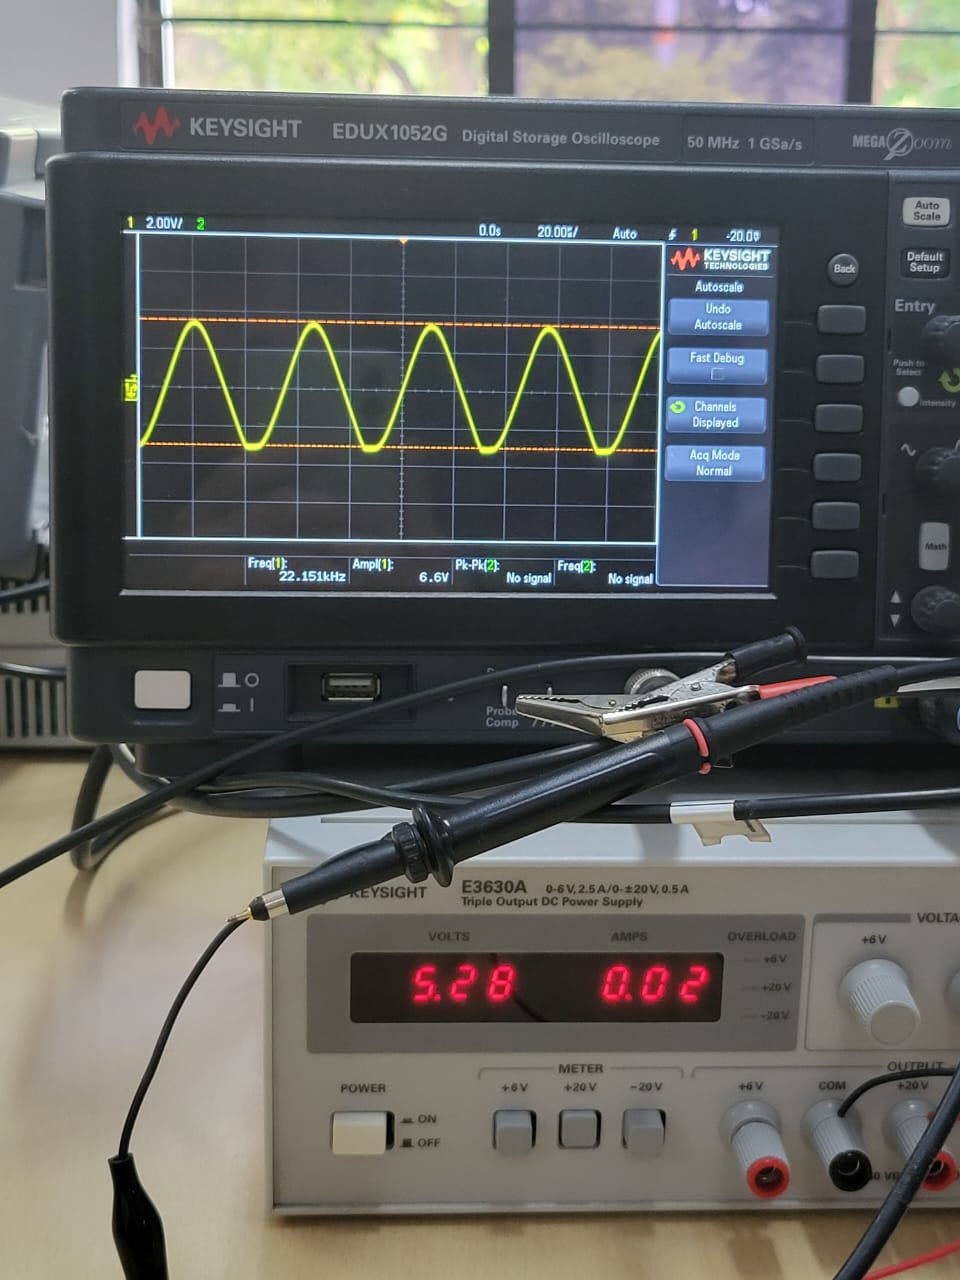
\includegraphics[width=0.9\linewidth]{fixed.jpeg} % Ensure this image file is present
    \caption{Fixed Oscillator Output Waveform (Physical Measurement)}
    \label{fig:Fixed_Oscillator}
\end{figure}

\section{Signal Processing Stages}

\subsection{Mixer (Summing Amplifier)}
The mixer combines the VFO and FFO signals to generate the sum and difference frequencies.
\begin{itemize}
    \item \textbf{Topology}: An inverting summing amplifier using U2 (OP27).
    \item \textbf{Key Components}: U2 (OP27), Input Resistors R4=\SI{47}{\kilo\ohm} (from VFO), R5=\SI{47}{\kilo\ohm} (from FFO), Feedback Resistor R6=\SI{20}{\kilo\ohm}.
    \item \textbf{Operation}: The output voltage is the inverted sum of the input voltages, scaled by the ratio of feedback to input resistance.
    \item \textbf{Gain Calculation}: The gain for each input is:
        \begin{equation}
            G = -\frac{R_f}{R_{in}} = -\frac{\SI{20}{\kilo\ohm}}{\SI{47}{\kilo\ohm}} \approx -0.426
        \end{equation}
    \item \textbf{Output Voltage}:
        \begin{equation}
            V_{out, mixer} = G \times (V_{VFO} + V_{FFO}) = -0.426 (V_{VFO} + V_{FFO})
        \end{equation}
        This output contains components at frequencies $f_{VFO}$, $f_{FFO}$, $f_{VFO}+f_{FFO}$, and $|f_{VFO}-f_{FFO}|$.
\end{itemize}

\subsection{Envelope Detector}
An envelope detector stage is included after the mixer. In traditional Theremins, envelope detection might relate to volume control coming from the second antenna. However, in our design, it is used to demodulate the mixed signal.
\begin{itemize}
    \item \textbf{Components}: Diode D (1N4148), R7 (\SI{10}{\kilo\ohm}), C2 (\SI{47}{\nano\farad}).
    \item \textbf{Function}: Performs half-wave rectification (via Diode D) followed by RC low-pass filtering (R7, C2) to extract the signal envelope \cite{envelope_ref}. This stage seems intended to demodulate the mixed signal to some extent, although its placement after the summing mixer is unconventional for isolating the beat frequency directly.
    \item \textbf{Time Constant}: $\tau = R7 \times C2 = (\SI{10}{\kilo\ohm})(\SI{47}{\nano\farad}) = \SI{0.47}{\milli\second}$.
    \item \textbf{Cutoff Frequency}: The RC filter has a cutoff frequency $f_c = \frac{1}{2\pi \tau} \approx \frac{1}{2\pi (\SI{0.47}{\milli\second})} \approx \SI{339}{\hertz}$. This low cutoff will primarily passes the lower frequency components, including the beat frequency, while smoothing the waveform. ( Note: Explained more in the youtube video \cite{project_video} )
\end{itemize}
The output after the envelope detector stage is shown in Fig.~\ref{fig:envelopeoutput}.

\begin{figure}[htbp]
    \centering
    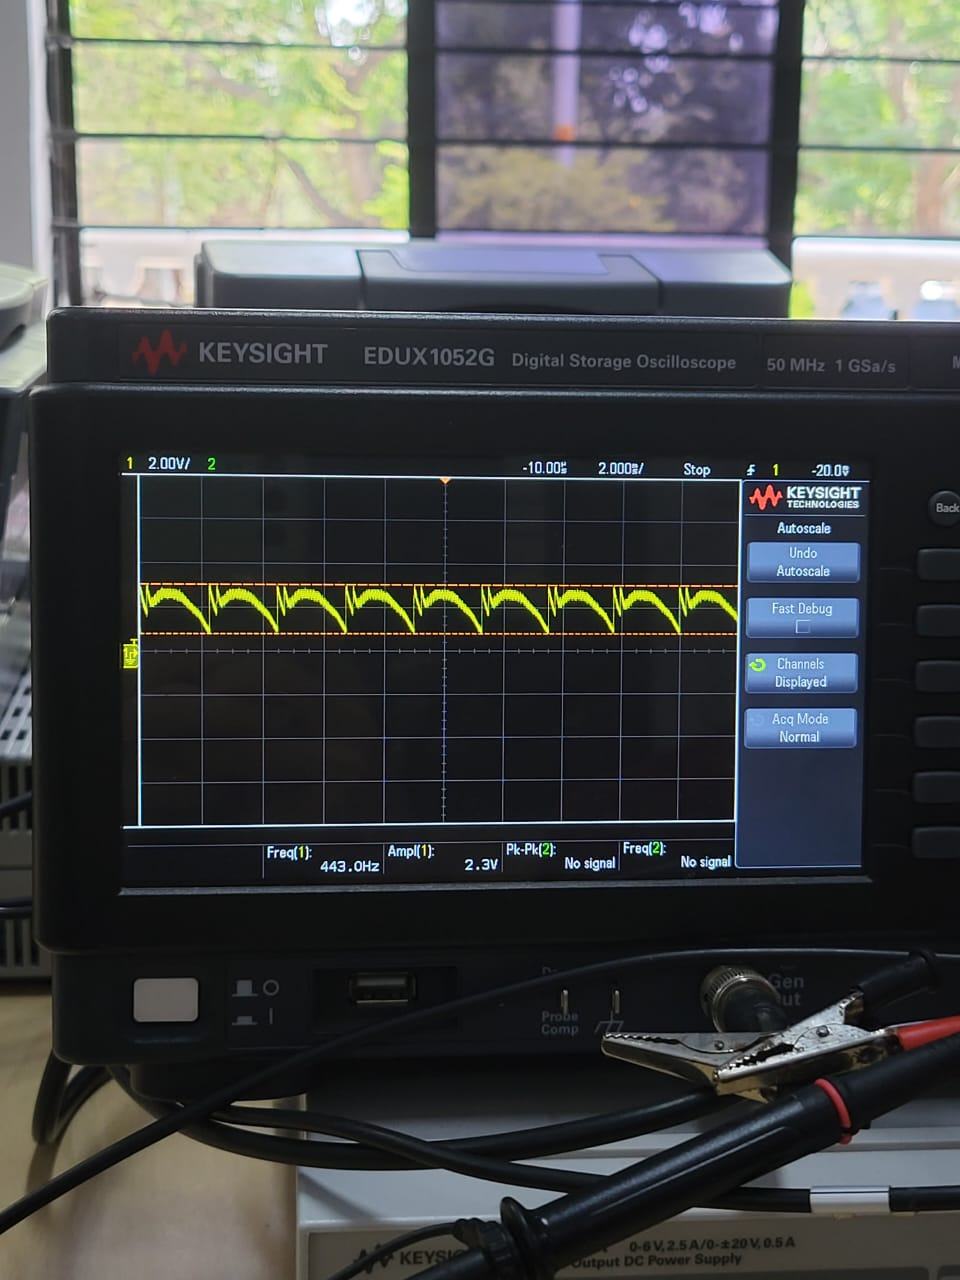
\includegraphics[width=0.3\textheight, keepaspectratio]{envelopeoutput.jpeg} % Ensure image file is present
    \caption{Envelope Detector Output Waveform (Physical Measurement)}
    \label{fig:envelopeoutput}
\end{figure}

\subsection{Active Filtering Stages}
Subsequent filtering stages refine the audio signal.

\subsubsection{Active High-Pass Filter (HPF)}
This filter removes any DC offset introduced by previous stages (like the envelope detector) and very low frequencies.
\begin{itemize}
    \item \textbf{Topology}: First-order active HPF using U3 (OP27) configured as a buffer.
    \item \textbf{Components}: U3 (OP27), C5 (\SI{4.7}{\nano\farad}), R13 (\SI{1.7}{\mega\ohm}).
    \item \textbf{Cutoff Frequency}:
        \begin{equation}
            f_{c, HPF} = \frac{1}{2\pi R13 C5} = \frac{1}{2\pi (\SI{1.7}{\mega\ohm})(\SI{4.7}{\nano\farad})} \approx \SI{19.9}{\hertz}
        \end{equation}
        This cutoff is appropriate for passing the audible range while blocking DC.
\end{itemize}
The output after the high-pass filter stage is shown in Fig.~\ref{fig:highpass}.

\begin{figure}[htbp]
    \centering
    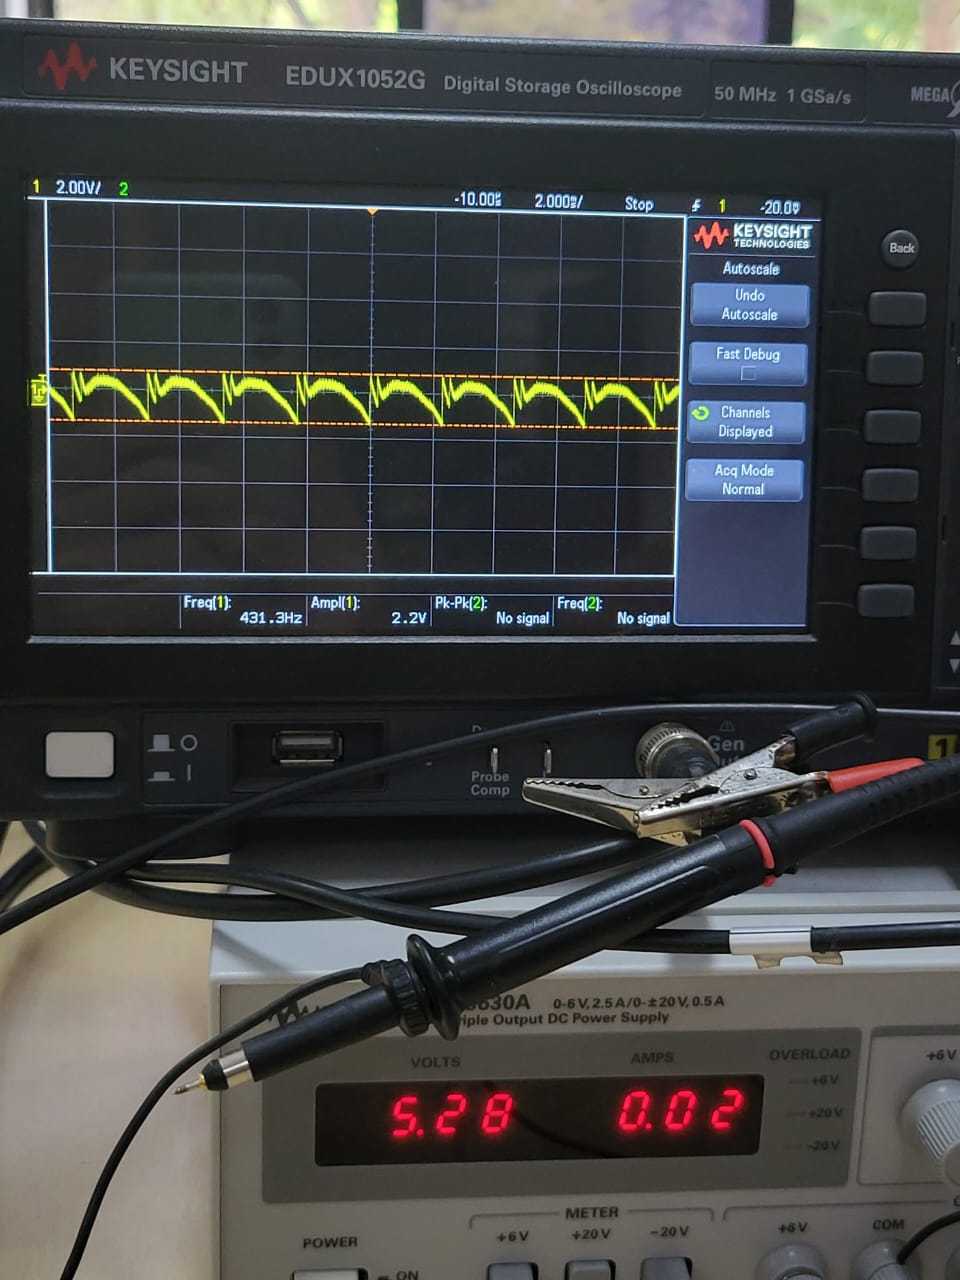
\includegraphics[width=0.8\linewidth]{highpass.jpeg} % Ensure image file is present
    \caption{High-Pass Filter Output Waveform (Physical Measurement)}
    \label{fig:highpass}
\end{figure}

\subsubsection{Active Low-Pass Filter (LPF)}
This filter removes high-frequency components remaining after mixing and envelope detection, such as sums of frequencies or oscillator harmonics, leaving primarily the desired difference frequency.
\begin{itemize}
    \item \textbf{Topology}: Second-order active LPF using U5 (OP27), likely a Sallen-Key or Multiple Feedback topology providing gain. Based on components R10, R11, R12, C3, R23, C9, it resembles a design with feedback providing amplification.
    \item \textbf{Components}: U5 (OP27), R10=\SI{6.3}{\kilo\ohm}, C3=\SI{10}{\nano\farad}, R23=\SI{6.3}{\kilo\ohm}, C9=\SI{10}{\nano\farad} (frequency determining); R11=\SI{40}{\kilo\ohm}, R12=\SI{20}{\kilo\ohm} (gain setting).
    \item \textbf{Cutoff Frequency Estimation}: For a Sallen-Key LPF with equal R (R10=R23) and C (C3=C9), $f_c = \frac{1}{2\pi RC}$. Using R=\SI{6.3}{\kilo\ohm} and C=\SI{10}{\nano\farad}:
        \begin{equation}
            f_{c, LPF} = \frac{1}{2\pi (\SI{6.3}{\kilo\ohm})(\SI{10}{\nano\farad})} \approx \SI{2.53}{\kilo\hertz}
        \end{equation}
    \item \textbf{DC Gain}: The gain appears set by R11 and R12 in a non-inverting configuration related to the feedback:
        \begin{equation}
             G_{DC} = 1 + \frac{R11}{R12} = 1 + \frac{\SI{40}{\kilo\ohm}}{\SI{20}{\kilo\ohm}} = 3
        \end{equation}
        This stage both filters and amplifies the audio signal.
\end{itemize}

\section{Amplification Stages}

\subsection{Pre-Amplifier / Volume Control}
This stage provides further voltage gain and incorporates the user volume control.
\begin{itemize}
    \item \textbf{Topology}: Non-inverting amplifier using U6 (OP27) with gain adjusted by potentiometer U9.
    \item \textbf{Components}: U6 (OP27), R14 (\SI{20}{\kilo\ohm}), R15 (\SI{5}{\kilo\ohm}), U9 (Potentiometer, \SI{10}{\kilo\ohm}).
    \item \textbf{Gain Range}: The voltage gain $A_v$ varies with the potentiometer setting ($R_{U9}$ represents the resistance from the wiper to ground):
        \begin{equation}
            A_v = 1 + \frac{R14}{R15 + R_{U9}}
        \end{equation}
        \begin{itemize}
            \item Minimum Gain ($R_{U9}=\SI{10}{\kilo\ohm}$): $A_v = 1 + \frac{20}{5 + 10} = 1 + \frac{20}{15} \approx 2.33$
            \item Maximum Gain ($R_{U9}=\SI{0}{\kilo\ohm}$): $A_v = 1 + \frac{20}{5 + 0} = 1 + 4 = 5$
        \end{itemize}
\end{itemize}

\subsection{Sound Amplifier}
An additional amplifier stage boosts the signal level before the power amplifier.
\begin{itemize}
    \item \textbf{Topology}: Inverting amplifier configuration using U4 (OP37).
    \item \textbf{Components}: U4 (OP37), R8 (\SI{10}{\kilo\ohm}), R9 (\SI{40}{\kilo\ohm}).
    \item \textbf{Gain}:
        \begin{equation}
            G = -\frac{R9}{R8} = -\frac{\SI{40}{\kilo\ohm}}{\SI{10}{\kilo\ohm}} = -4
        \end{equation}
        This stage inverts the signal while providing a gain of 4.
\end{itemize}

\section{Power Amplifier Stage}
The final stage provides the necessary current to drive a low-impedance load like a speaker.
\begin{itemize}
    \item \textbf{Topology}: Class AB Push-Pull output stage using complementary BJT pair.
    \item \textbf{Key Components}: Q1 (TIP31C NPN BJT), Q2 (TIP32C PNP BJT), D1, D2 (1N4148 diodes for bias), R20, R21 (\SI{1}{\kilo\ohm} base resistors), C7, C8 (\SI{1}{\micro\farad} bypass capacitors), R22 (\SI{10}{\ohm} load resistor).
    \item \textbf{Operation}: Q1 amplifies the positive half-cycles of the input signal, while Q2 amplifies the negative half-cycles. Diodes D1 and D2 provide a small forward bias voltage between the bases of Q1 and Q2 to minimize crossover distortion, ensuring a smoother transition between the transistors conducting. This stage primarily provides current gain (power gain) with approximately unity voltage gain.
\end{itemize}

\section{Power Supply}
The circuit requires a stable dual-rail power supply for the operational amplifiers and other stages.
\begin{itemize}
    \item \textbf{Requirement}: $\pm$ \SI{5}{\volt} DC.
    \item \textbf{Implementation}: Typically achieved using two 9V batteries connected in series with the center tap serving as ground. Voltage regulators LM7805 (for +5V) and LM7905 (for -5V) are used to provide stable regulated voltages from the batteries.
    \item \textbf{Consumption}: The Op-Amps consume relatively low quiescent current. The power amplifier stage draws more current depending on the output volume and load. The total power consumption is estimated to be under \SI{3}{\watt} under normal operation.
\end{itemize}

\section{Operation and Results}
The integrated Theremin circuit functions as follows: The player's hand proximity to the antenna (modeled by C$_{\text{Antenna}}$) controls the frequency of the VFO (U1). This signal is mixed (U2) with the stable frequency from the FFO (U7). The resulting mixed signal undergoes envelope detection (D, R7, C2) and active filtering (U3, U5) to isolate and clean up the audible difference frequency ($|f_{VFO} - f_{FFO}|$). This audio signal is then amplified (U6, U4), with volume controlled by the potentiometer (U9), and finally fed to the Class AB power amplifier (Q1, Q2) to drive the speaker (R22).

Physical measurements (Fig.~\ref{fig:Variable_Oscillator}, \ref{fig:Fixed_Oscillator}, \ref{fig:envelopeoutput}, \ref{fig:highpass}) confirm the operation of individual stages, showing the expected waveforms at the outputs of the oscillators, envelope detector, and high-pass filter. The variable oscillator frequency changes as intended with capacitance, and the fixed oscillator provides a stable reference. The filtering stages shape the signal towards the final audio output. The overall result is an audible tone whose pitch changes with hand movement near the antenna and whose volume is adjustable via the potentiometer.

\section{Project Demonstration}
A video demonstration showcasing the operation of the constructed Theremin circuit is available online \cite{project_video}. The video explains the working principles, shows the physical circuit build, and demonstrates the pitch control via hand proximity to the antenna and volume control using the potentiometer.

\section{Conclusion}
This project successfully demonstrated the design, simulation, and testing of an electronic Theremin circuit based on operational amplifiers and a BJT Class AB output stage. The design employs the principle of heterodyning by mixing signals from a hand-capacitance controlled Variable Frequency Oscillator and a Fixed Frequency Oscillator (Wien Bridge type). The resulting difference frequency is extracted using an envelope detector and active filtering stages (high-pass and low-pass) to produce an audible tone within the range of approximately \SI{20}{Hz} to \SI{2.5}{kHz} (based on filter cutoffs).

Volume control is implemented manually via a potentiometer integrated into a pre-amplifier stage. A final Class AB power amplifier provides sufficient power to drive a standard \SI{10}{\ohm} speaker load. The circuit operates from a standard $\pm$\SI{5}{\volt} regulated dual power supply. The design choices, particularly the use of an envelope detector post-mixing and potentiometer-based volume control, differ from some traditional Theremin architectures but provide a functional implementation of the core concept. The simulation and physical measurements validate the operation of the individual stages and the overall system.

% Add references if needed, using the links from the slides
\begin{thebibliography}{9}
\bibitem{theremin_wiki} Wikipedia contributors, "Theremin," Wikipedia, The Free Encyclopedia, \url{https://en.wikipedia.org/wiki/Theremin} .
\bibitem{relax_osc} Circuit Digest, "Relaxation Oscillator using Op-Amp," \url{https://circuitdigest.com/tutorial/relaxation-oscillator-using-op-amp} .
\bibitem{envelope_ref} C. Rose, "Envelope Detector," Rutgers WINLAB, \url{https://www.winlab.rutgers.edu/~crose/322_html/envelope_detector.html} .
\bibitem{project_video} K. Pandya and V. Wadhwani, "Theremin Project Explanation and Demo," YouTube, May 5, 2025. [Online]. Available: \url{https://youtu.be/XMQbpG15ijk?si=fTLJ23zKhtOCA8q9}
\bibitem{Github} K. Pandya and V. Wadhwani, "Theremin Project GitHub Repository," \url{https://github.com/MostlyKIGuess/theremin-circuit} .

% Add other references if necessary
\end{thebibliography}

\end{document}